\documentclass[11pt]{article}

\usepackage[margin=1in]{geometry}
\usepackage{amsmath,amssymb,amsthm}
\usepackage{bm}
\usepackage{booktabs}
\usepackage{tikz}
\usetikzlibrary{arrows.meta,calc,angles,quotes}
\usepackage{pgfplots}
\pgfplotsset{compat=1.18}
\usepackage{listings}
\usepackage{xcolor}
\usepackage[hidelinks]{hyperref}
\usepackage{enumitem}

\definecolor{teal}{HTML}{1D9E75}
\definecolor{purp}{HTML}{534AB7}
\definecolor{coral}{HTML}{D85A30}
\definecolor{amber}{HTML}{EF9F27}
\definecolor{slate}{HTML}{888780}
\definecolor{redd}{HTML}{E24B4A}

\lstset{
  basicstyle=\ttfamily\small,
  breaklines=true,
  frame=single,
  rulecolor=\color{slate},
  columns=fullflexible,
  keywordstyle=\color{purp},
  commentstyle=\color{slate}\itshape,
  stringstyle=\color{coral},
  showstringspaces=false
}

\newtheorem{proposition}{Proposition}
\newtheorem{lemma}{Lemma}
\theoremstyle{definition}
\newtheorem{definition}{Definition}
\theoremstyle{remark}
\newtheorem{remark}{Remark}

\newcommand{\vb}[1]{\bm{#1}}
\newcommand{\uv}[1]{\hat{\bm{#1}}}
\newcommand{\Es}{E_{\pm}}
\newcommand{\Eu}{E_{\cos}}
\newcommand{\SJ}{\mathrm{SJ}}

\title{Dihedral Angles, Scaled Jacobians, and a Signed Corner Energy\\
\large for Hexahedral Finite Element Meshes}
\author{Notes compiled from a working session with Claude (Anthropic)}
\date{October 8, 2026}

\begin{document}
\maketitle

\begin{abstract}
These notes collect, formalize, and derive the results developed in an interactive
session on mesh-quality geometry. We first derive the dihedral angle between two
triangular facets that share an edge. We then derive the scaled Jacobian (SJ) at a
corner of a trilinear hexahedral element and show that it equals the signed volume of
the parallelepiped spanned by the three unit edge vectors. We introduce an
orthogonality-based \emph{corner energy}, $\Eu=\sum\cos^2\theta_{ij}$, and show that it
is blind to element inversion. We then construct a \emph{signed corner energy}
$\Es=\sum_k(1-\uv{e}_k\cdot\uv{n}_{ij})$ that vanishes only at a perfect right-handed
corner, equals $3$ exactly at degeneracy, and keeps increasing as the corner inverts.
All formulas are derived in full, the one-parameter test configuration used in the
interactive illustrations is solved in closed form, and practical notes on embedding
the illustrations in an mdBook are included. A record of the conversation is given in
Appendix~\ref{app:conversation}.
\end{abstract}

\tableofcontents
\newpage

%=====================================================================
\section{Notation}
%=====================================================================

Vectors are bold ($\vb{a}$); unit vectors carry a hat, $\uv{a}=\vb{a}/\|\vb{a}\|$.
For two nonzero vectors, the (unsigned) angle between them is
\begin{equation}
  \theta(\vb{a},\vb{b}) = \arccos\!\left(\frac{\vb{a}\cdot\vb{b}}{\|\vb{a}\|\,\|\vb{b}\|}\right)\in[0,\pi].
\end{equation}
Two identities are used repeatedly:
\begin{align}
  \|\vb{a}\times\vb{b}\| &= \|\vb{a}\|\,\|\vb{b}\|\sin\theta(\vb{a},\vb{b}), \label{eq:crossnorm}\\
  (\vb{a}\times\vb{b})\cdot(\vb{c}\times\vb{d}) &= (\vb{a}\cdot\vb{c})(\vb{b}\cdot\vb{d})-(\vb{a}\cdot\vb{d})(\vb{b}\cdot\vb{c}) \quad\text{(Binet--Cauchy).} \label{eq:binet}
\end{align}
The scalar triple product $[\vb{a},\vb{b},\vb{c}]=\vb{a}\cdot(\vb{b}\times\vb{c})=\det[\vb{a}\;\vb{b}\;\vb{c}]$
is invariant under cyclic permutation and changes sign under any transposition:
\begin{equation}
  [\vb{a},\vb{b},\vb{c}] = [\vb{b},\vb{c},\vb{a}] = [\vb{c},\vb{a},\vb{b}] = -[\vb{b},\vb{a},\vb{c}].
  \label{eq:cyclic}
\end{equation}

%=====================================================================
\section{The dihedral angle between two triangular facets}
%=====================================================================

\subsection{Definition}

Let two triangles $T_1=(A,B,P)$ and $T_2=(A,B,Q)$ share the edge $AB$, with apexes
$P$ and $Q$ on (generally) different sides. The \emph{dihedral angle} $\theta$ between
them is the angle between the two half-planes bounded by line $AB$, measured in a plane
perpendicular to $AB$.

\begin{figure}[h]
\centering
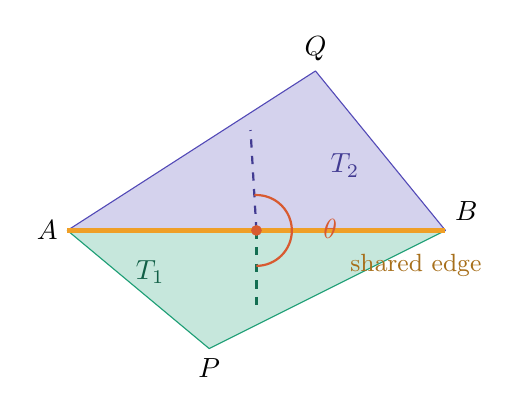
\begin{tikzpicture}[scale=1.5,line join=round]
  % oblique projection: edge AB along x; face 1 tilted toward viewer, face 2 up-back
  \coordinate (A) at (-1.6,0);
  \coordinate (B) at (1.6,0);
  \coordinate (P) at (-0.4,-1.0);
  \coordinate (Q) at (0.5,1.35);
  \coordinate (M) at (0,0);
  \filldraw[fill=teal!25,draw=teal] (A)--(B)--(P)--cycle;
  \filldraw[fill=purp!25,draw=purp] (A)--(B)--(Q)--cycle;
  \draw[amber,line width=2pt] (A)--(B);
  \draw[teal!70!black,dashed,thick] (M)--(0.0,-0.68) coordinate (U);
  \draw[purp!80!black,dashed,thick] (M)--(-0.05,0.85) coordinate (V);
  \pic[draw=coral,thick,angle radius=0.45cm,"$\theta$"{coral,anchor=west},angle eccentricity=1.6] {angle=U--M--V};
  \fill[coral] (M) circle (1.3pt);
  \node[left] at (A) {$A$};
  \node[above right] at (B) {$B$};
  \node[below] at (P) {$P$};
  \node[above] at (Q) {$Q$};
  \node[teal!60!black] at (-0.9,-0.35) {$T_1$};
  \node[purp!80!black] at (0.75,0.55) {$T_2$};
  \node[below,font=\small,amber!70!black] at (1.35,-0.12) {shared edge};
\end{tikzpicture}
\caption{Two facets hinged on a shared edge. The dashed rays lie in each face and are
perpendicular to the edge at a common point; the angle between them is the dihedral
angle $\theta$.}
\label{fig:dihedral}
\end{figure}

\subsection{Derivation via perpendicular rays}

Let $\uv{t}=(B-A)/\|B-A\|$ be the unit edge direction. Remove the component of each
apex offset along the edge:
\begin{equation}
  \vb{u} = (P-A) - \big((P-A)\cdot\uv{t}\big)\uv{t},\qquad
  \vb{v} = (Q-A) - \big((Q-A)\cdot\uv{t}\big)\uv{t}.
  \label{eq:uv}
\end{equation}
By construction $\vb{u}\perp\uv{t}$ and $\vb{u}$ lies in the plane of $T_1$ (it is a
linear combination of $P-A$ and $B-A$); likewise for $\vb{v}$ and $T_2$. Hence $\vb{u}$ and
$\vb{v}$ are exactly the perpendicular rays of Figure~\ref{fig:dihedral}, and
\begin{equation}
  \boxed{\cos\theta = \frac{\vb{u}\cdot\vb{v}}{\|\vb{u}\|\,\|\vb{v}\|}.}
  \label{eq:dihedral-uv}
\end{equation}

\subsection{Derivation via face normals}

Define face normals with a consistent ``from the edge toward the face'' orientation:
$\vb{n}_1 = \uv{t}\times\vb{u}$ and $\vb{n}_2=\uv{t}\times\vb{v}$. By the Binet--Cauchy
identity~\eqref{eq:binet},
\begin{equation}
  \vb{n}_1\cdot\vb{n}_2 = (\uv{t}\cdot\uv{t})(\vb{u}\cdot\vb{v}) - (\uv{t}\cdot\vb{v})(\vb{u}\cdot\uv{t})
  = \vb{u}\cdot\vb{v},
\end{equation}
since $\uv{t}\cdot\uv{t}=1$ and $\uv{t}\cdot\vb{u}=\uv{t}\cdot\vb{v}=0$. Also
$\|\vb{n}_1\|=\|\vb{u}\|$ and $\|\vb{n}_2\|=\|\vb{v}\|$ by~\eqref{eq:crossnorm}, since
$\vb{u}\perp\uv{t}$. Therefore, with these normals, $\cos\theta=\uv{n}_1\cdot\uv{n}_2$.

In a closed, consistently oriented surface the \emph{outward} normals of two
adjacent faces are $\vb{n}_1^{\text{out}}=\pm\vb{n}_1$ and $\vb{n}_2^{\text{out}}=\mp\vb{n}_2$
(one face is traversed in each direction across the shared edge). Hence
\begin{equation}
  \boxed{\cos\theta = -\,\frac{\vb{n}^{\text{out}}_1\cdot\vb{n}^{\text{out}}_2}{\|\vb{n}^{\text{out}}_1\|\,\|\vb{n}^{\text{out}}_2\|}}
  \quad\text{(both outward or both inward)},
  \label{eq:dihedral-normals}
\end{equation}
and the sign flips if one normal points in and the other out. Limiting cases: $\theta=\pi$
means the facets are coplanar (flat); $\theta\to 0$ means they fold shut.

\subsection{Robust and signed evaluation}

Because $\arccos$ is ill-conditioned near $0$ and $\pi$, a numerically robust form is
\begin{equation}
  \theta = \operatorname{atan2}\!\big(\|\vb{u}\times\vb{v}\|,\;\vb{u}\cdot\vb{v}\big)\in[0,\pi].
\end{equation}
A \emph{signed} dihedral angle in $(-\pi,\pi]$, distinguishing which way $T_2$ is
rotated relative to $T_1$ about $\uv{t}$, is
\begin{equation}
  \theta_{\text{signed}} = \operatorname{atan2}\!\big((\vb{u}\times\vb{v})\cdot\uv{t},\;\vb{u}\cdot\vb{v}\big).
\end{equation}

\begin{remark}
Viewing the configuration straight down the shared edge is the one viewpoint in which
the on-screen angle equals $\theta$, because that view is the plane perpendicular to
$\uv{t}$ seen head-on. This is the behavior demonstrated by the interactive illustration.
\end{remark}

%=====================================================================
\section{The scaled Jacobian at a hexahedral corner}
%=====================================================================

\subsection{From the trilinear map to edge vectors}

A trilinear hexahedron maps the reference cube $[-1,1]^3\ni\bm{\xi}=(\xi,\eta,\zeta)$ to
physical space by
\begin{equation}
  \vb{x}(\bm{\xi}) = \sum_{a=1}^{8} N_a(\bm{\xi})\,\vb{x}_a,\qquad
  N_a(\bm{\xi}) = \tfrac18(1+\xi_a\xi)(1+\eta_a\eta)(1+\zeta_a\zeta),
\end{equation}
where $(\xi_a,\eta_a,\zeta_a)\in\{\pm1\}^3$ are the reference coordinates of node $a$.
The Jacobian matrix is $J=\partial\vb{x}/\partial\bm{\xi}$.

\begin{lemma}\label{lem:cornerJ}
At a corner node $a$, the columns of $J$ are one half of the three edge vectors leaving
that node (oriented along increasing $\xi,\eta,\zeta$ reference directions).
\end{lemma}
\begin{proof}
Take the corner $\bm{\xi}_0=(-1,-1,-1)$ with node $\vb{x}_0$ and neighbors $\vb{x}_\xi,\vb{x}_\eta,\vb{x}_\zeta$
along the three reference axes. On the reference edge $\eta=\zeta=-1$ every shape
function except those of $\vb{x}_0$ and $\vb{x}_\xi$ vanishes, and the map reduces to
$\vb{x}(\xi,-1,-1)=\tfrac12(1-\xi)\vb{x}_0+\tfrac12(1+\xi)\vb{x}_\xi$. Its derivative is
$\partial\vb{x}/\partial\xi=\tfrac12(\vb{x}_\xi-\vb{x}_0)$, and the same holds for $\eta$ and $\zeta$.
Since the partial derivative along $\xi$ evaluated at a point on that edge depends only on the
restriction of $\vb{x}$ to the edge, these are the columns of $J(\bm{\xi}_0)$. Other corners follow by
symmetry, with edge vectors oriented along the increasing reference directions.
\end{proof}

Writing $\vb{e}_1,\vb{e}_2,\vb{e}_3$ for the three edge vectors at the corner (ordered so that the
reference frame $(\xi,\eta,\zeta)$ is right-handed), Lemma~\ref{lem:cornerJ} gives
\begin{equation}
  \det J = \tfrac18\,[\vb{e}_1,\vb{e}_2,\vb{e}_3].
\end{equation}

\subsection{Scaling}

\begin{definition}[Corner scaled Jacobian]
\begin{equation}
  \boxed{\SJ = \frac{[\vb{e}_1,\vb{e}_2,\vb{e}_3]}{\|\vb{e}_1\|\,\|\vb{e}_2\|\,\|\vb{e}_3\|}
  = \uv{e}_1\cdot(\uv{e}_2\times\uv{e}_3) = \det\big[\uv{e}_1\;\uv{e}_2\;\uv{e}_3\big].}
  \label{eq:SJ}
\end{equation}
\end{definition}
The factor $\tfrac18$ cancels against the same factor in the edge lengths of $J$'s columns,
so~\eqref{eq:SJ} is the determinant of $J$ with its columns normalized.

\paragraph{Geometric meaning.} $|[\uv{e}_1,\uv{e}_2,\uv{e}_3]|$ is the volume of the
parallelepiped spanned by the three \emph{unit} edges, and the sign records orientation:
positive for a right-handed corner, negative for a left-handed (inverted) one.

\begin{proposition}[Range]\label{prop:SJrange}
$-1\le\SJ\le 1$, with $\SJ=1$ if and only if the unit edges form a right-handed
orthonormal triad, and $\SJ=-1$ if and only if they form a left-handed one.
\end{proposition}
\begin{proof}
Write $\uv{n}=\uv{e}_2\times\uv{e}_3$. By~\eqref{eq:crossnorm},
$\|\uv{n}\|=\sin\theta_{23}\le 1$, so by Cauchy--Schwarz
$|\SJ|=|\uv{e}_1\cdot\uv{n}|\le\|\uv{n}\|\le 1$ (Hadamard's inequality for this case).
Equality $|\SJ|=1$ requires both $\sin\theta_{23}=1$ (so $\uv{e}_2\perp\uv{e}_3$) and
$\uv{e}_1\parallel\uv{n}$ (so $\uv{e}_1\perp\uv{e}_2,\uv{e}_3$), i.e.\ an orthonormal triad;
the sign of $\uv{e}_1\cdot\uv{n}$ is its handedness.
\end{proof}

\paragraph{Element minimum.} The element's minimum scaled Jacobian is
$\mathrm{MSJ}=\min_{a=1..8}\SJ_a$ over its eight corners (some implementations also include
the element center). A single bad corner therefore sets the element's MSJ.

\begin{table}[h]
\centering
\begin{tabular}{@{}lll@{}}
\toprule
Regime & $\SJ$ & Geometry at the corner \\
\midrule
Ideal & $1$ & orthonormal, right-handed: a cube corner \\
Valid but distorted & $(0,1)$ & positive volume, skewed edges \\
Degenerate & $0$ & the three edges are coplanar; zero volume; $J$ singular \\
Inverted & $<0$ & left-handed; negative volume; element folded \\
Fully reflected & $-1$ & orthonormal, left-handed \\
\bottomrule
\end{tabular}
\caption{Regimes of the corner scaled Jacobian.}
\end{table}

%=====================================================================
\section{The one-parameter test configuration}
\label{sec:config}
%=====================================================================

The interactive illustrations use a two-parameter family of corners. Place $\vb{e}_1$ and
$\vb{e}_2$ in the $xy$-plane separated by the base angle $\varphi\in(0,\pi)$, and tilt
$\vb{e}_3$ out of that plane by the elevation $\alpha\in[-\pi,\pi]$ while keeping its
azimuth on the bisector $\beta=\varphi/2$:
\begin{equation}
  \uv{e}_1=\begin{pmatrix}1\\0\\0\end{pmatrix},\quad
  \uv{e}_2=\begin{pmatrix}\cos\varphi\\\sin\varphi\\0\end{pmatrix},\quad
  \uv{e}_3=\begin{pmatrix}\cos\alpha\cos\beta\\\cos\alpha\sin\beta\\\sin\alpha\end{pmatrix},\quad
  \beta=\tfrac{\varphi}{2}.
  \label{eq:config}
\end{equation}
The perfect corner is $\varphi=\alpha=\pi/2$. For $\alpha\in(\pi/2,\pi]$ the edge $\uv{e}_3$
tips over the top and leans toward the opposite side; at $\alpha=\pm\pi$ it lies in the base
plane, and at $\alpha=-\pi/2$ it points straight down. Throughout, write
\begin{equation}
  s=\sin\alpha,\qquad h=\cos\tfrac{\varphi}{2},\qquad \sigma=\sin\tfrac{\varphi}{2}.
\end{equation}

\subsection{Pairwise angles}

\begin{align}
  \cos\theta_{12} &= \uv{e}_1\cdot\uv{e}_2=\cos\varphi, \label{eq:c12}\\
  \cos\theta_{13} &= \uv{e}_1\cdot\uv{e}_3=\cos\alpha\cos\beta=\cos\alpha\,h, \label{eq:c13}\\
  \cos\theta_{23} &= \uv{e}_2\cdot\uv{e}_3=\cos\alpha(\cos\varphi\cos\beta+\sin\varphi\sin\beta)
                    =\cos\alpha\cos(\varphi-\beta)=\cos\alpha\,h. \label{eq:c23}
\end{align}
So placing $\uv{e}_3$ on the bisector makes $\theta_{13}=\theta_{23}$ for every $\alpha$.

\subsection{Scaled Jacobian}

$\uv{e}_1\times\uv{e}_2=(0,0,\sin\varphi)^{\mathsf T}$, so by cyclicity~\eqref{eq:cyclic}
\begin{equation}
  \boxed{\SJ(\alpha,\varphi)=(\uv{e}_1\times\uv{e}_2)\cdot\uv{e}_3=\sin\varphi\,\sin\alpha = s\sin\varphi.}
  \label{eq:SJconfig}
\end{equation}
$\SJ$ is the product of two factors: base skew ($\sin\varphi$) and out-of-plane tilt
($\sin\alpha$). It vanishes exactly when $\alpha\in\{0,\pm\pi\}$ (with $0<\varphi<\pi$) and is negative
exactly when $\alpha\in(-\pi,0)$.

\begin{remark}[Symmetry]
Every quantity in this configuration depends on $\alpha$ only through $s=\sin\alpha$ and
$\cos^2\alpha=1-s^2$ (see~\eqref{eq:c13}--\eqref{eq:Esconfig}). All curves are therefore symmetric
about $\alpha=\pi/2$ (and about $\alpha=-\pi/2$) on the full interval $[-\pi,\pi]$.
\end{remark}

%=====================================================================
\section{An orthogonality corner energy and its blind spot}
%=====================================================================

\begin{definition}[Unsigned corner energy]
\begin{equation}
  \boxed{\Eu=\cos^2\theta_{12}+\cos^2\theta_{13}+\cos^2\theta_{23}
   =(\uv{e}_1\cdot\uv{e}_2)^2+(\uv{e}_1\cdot\uv{e}_3)^2+(\uv{e}_2\cdot\uv{e}_3)^2.}
\end{equation}
\end{definition}

Each term is $0$ exactly when that pair is at $90^\circ$ and rises smoothly as the pair
departs from $90^\circ$. Hence $\Eu\ge0$, $\Eu=0$ iff all three pairs are orthogonal, and
$\Eu\le3$ with equality iff all edges are parallel or antiparallel.

\paragraph{In the test configuration.} From~\eqref{eq:c12}--\eqref{eq:c23},
\begin{equation}
  \Eu(\alpha,\varphi)=\cos^2\varphi+2\cos^2\alpha\cos^2\tfrac{\varphi}{2}
  =\cos^2\varphi+2(1-s^2)h^2.
  \label{eq:Euconfig}
\end{equation}

\begin{proposition}[Inversion blindness]\label{prop:blind}
$\Eu$ is invariant under $\uv{e}_k\mapsto-\uv{e}_k$ for any single edge, and more generally under
any reflection of the triad. In particular $\Eu$ cannot distinguish a perfect corner
($\SJ=1$) from a fully reflected one ($\SJ=-1$): both have $\Eu=0$.
\end{proposition}
\begin{proof}
Each term $(\uv{e}_i\cdot\uv{e}_j)^2$ is even in each argument and invariant under orthogonal
maps, including reflections. Reflecting $\uv{e}_3\mapsto-\uv{e}_3$ in the perfect corner gives an
orthonormal left-handed triad.
\end{proof}

Along the test family with $\varphi=\pi/2$, $\Eu=\cos^2\alpha$: it rises from $0$ at $\alpha=\pi/2$
to $1$ at the degenerate corner $\alpha=0$, then \emph{falls back} to $0$ as the corner
inverts toward $\alpha=-\pi/2$. Over the full range $[-\pi,\pi]$ it has two equal minima, at
$\pm\pi/2$, rating the perfect and the fully reflected corners as equally good.

\paragraph{Root cause.} $\cos^2\theta$ is an \emph{even} function of the reflection
$\psi\mapsto\pi-\psi$ of an edge across a plane. Any energy built only from unsigned angles
inherits this blindness. To break the symmetry the energy must contain a quantity that is
\emph{odd} under reflection---i.e.\ it must involve orientation, which in three dimensions
means a cross product (equivalently, the triple product that defines the Jacobian).

%=====================================================================
\section{A signed corner energy}
%=====================================================================

\subsection{Definition}

For each edge $k$, let $(i,j,k)$ be the cyclic ordering $(1,2,3),(2,3,1),(3,1,2)$ and
define the oriented unit normal of the plane of the other two edges,
\begin{equation}
  \uv{n}_{ij}=\frac{\uv{e}_i\times\uv{e}_j}{\|\uv{e}_i\times\uv{e}_j\|},
\end{equation}
and let $\psi_k\in[0,\pi]$ be the angle between $\uv{e}_k$ and $\uv{n}_{ij}$.

\begin{definition}[Signed corner energy]
\begin{equation}
  \boxed{\Es=\sum_{k=1}^{3}\big(1-\cos\psi_k\big)=\sum_{(i,j,k)\,\text{cyclic}}\big(1-\uv{e}_k\cdot\uv{n}_{ij}\big).}
  \label{eq:Es}
\end{equation}
\end{definition}

The function $1-\cos\psi$ is strictly increasing on $[0,\pi]$ and is \emph{not} symmetric under
$\psi\mapsto\pi-\psi$; this is precisely what restores orientation awareness. Equivalently,
$1-\cos\psi_k=2\sin^2(\psi_k/2)$.

\subsection{Relation to the scaled Jacobian}

\begin{lemma}\label{lem:link}
For every cyclic $(i,j,k)$,
\begin{equation}
  \uv{e}_k\cdot\uv{n}_{ij}=\frac{\SJ}{\sin\theta_{ij}},
\end{equation}
and hence
\begin{equation}
  \boxed{\Es=\sum_{(i,j)}\left(1-\frac{\SJ}{\sin\theta_{ij}}\right)
  =3-\SJ\left(\frac{1}{\sin\theta_{12}}+\frac{1}{\sin\theta_{23}}+\frac{1}{\sin\theta_{31}}\right).}
  \label{eq:Eslink}
\end{equation}
\end{lemma}
\begin{proof}
By~\eqref{eq:crossnorm}, $\|\uv{e}_i\times\uv{e}_j\|=\sin\theta_{ij}$. By cyclicity~\eqref{eq:cyclic},
$\uv{e}_k\cdot(\uv{e}_i\times\uv{e}_j)=[\uv{e}_k,\uv{e}_i,\uv{e}_j]=[\uv{e}_1,\uv{e}_2,\uv{e}_3]=\SJ$ for each
cyclic $(i,j,k)$. Divide.
\end{proof}

So $\Es$ is the scaled Jacobian reweighted by the inverse sines of the three face
angles at the corner: it penalizes skew (small $\sin\theta_{ij}$) and inversion (negative $\SJ$)
through a single quantity.

\subsection{Properties}

\begin{proposition}\label{prop:Esprops}
Assume no two edges are parallel ($\sin\theta_{ij}>0$). Then
\begin{enumerate}[label=(\roman*)]
  \item $0\le\Es\le6$;
  \item $\Es=0$ if and only if the corner is perfect (orthonormal, right-handed, $\SJ=1$);
  \item $\Es=3$ if and only if $\SJ=0$ (degenerate), independently of the face angles;
  \item $\Es<3$ iff $\SJ>0$ and $\Es>3$ iff $\SJ<0$;
  \item $\Es=6$ if and only if the corner is orthonormal and left-handed ($\SJ=-1$).
\end{enumerate}
\end{proposition}
\begin{proof}
(i) Each $\cos\psi_k\in[-1,1]$, so each term lies in $[0,2]$.

(ii) $\Es=0$ iff every $\cos\psi_k=1$, i.e.\ $\uv{e}_k=\uv{n}_{ij}$ for all $k$. Then
$\uv{e}_3=\uv{n}_{12}\perp\uv{e}_1,\uv{e}_2$ and $\uv{e}_1=\uv{n}_{23}\perp\uv{e}_2$, so the triad is
orthonormal, and $\SJ=\uv{e}_3\cdot\uv{n}_{12}\sin\theta_{12}=1>0$. Conversely a right-handed
orthonormal triad has $\uv{e}_k=\uv{e}_i\times\uv{e}_j$ for every cyclic triple.

(iii)--(iv) From~\eqref{eq:Eslink}, $\Es-3=-\SJ\sum_{(i,j)}1/\sin\theta_{ij}$ and the sum is positive.

(v) Same as (ii) with $\uv{e}_k=-\uv{n}_{ij}$ for all $k$.
\end{proof}

Property (iii) is what makes $\Es$ a natural companion to $\SJ$: the degenerate threshold
$\SJ=0$ maps to the fixed threshold $\Es=3$ for every corner shape, and on each side the energy
is ordered by orientation.

\subsection{Closed form in the test configuration and monotonicity}

In the configuration~\eqref{eq:config}: $\sin\theta_{12}=\sin\varphi$, and from~\eqref{eq:c13}--\eqref{eq:c23},
\begin{equation}
  \sin\theta_{13}=\sin\theta_{23}=\sqrt{1-h^2\cos^2\alpha}=\sqrt{1-h^2(1-s^2)}=\sqrt{\sigma^2+h^2s^2}
  \equiv\sqrt{D(s)}.
\end{equation}
Substituting $\SJ=s\sin\varphi$ into~\eqref{eq:Eslink}:
\begin{equation}
  \boxed{\Es(\alpha,\varphi)=3-\sin\alpha-\frac{2\sin\varphi\,\sin\alpha}{\sqrt{\sin^2\frac{\varphi}{2}+\cos^2\frac{\varphi}{2}\sin^2\alpha}}
  =3-s-\frac{2s\sin\varphi}{\sqrt{D(s)}}.}
  \label{eq:Esconfig}
\end{equation}
(The first term after $3$ is the $\uv{e}_3$ term: $\uv{n}_{12}=\uv{z}$, so $\cos\psi_3=\sin\alpha$.)

\begin{proposition}[Monotone through inversion]\label{prop:mono}
For fixed $\varphi\in(0,\pi)$, $\Es$ is a strictly decreasing function of $s=\sin\alpha$ on $[-1,1]$.
Consequently, as $\uv{e}_3$ tilts from vertical ($\alpha=\pi/2$) down through the plane ($\alpha=0$)
and into inversion ($\alpha\to-\pi/2$), $\Es$ increases strictly and continuously, with no
turning point at $\SJ=0$.
\end{proposition}
\begin{proof}
Let $f(s)=s/\sqrt{D(s)}$ with $D(s)=\sigma^2+h^2s^2>0$. Then
\begin{equation}
  f'(s)=\frac{\sqrt{D}-s\cdot\frac{h^2s}{\sqrt{D}}}{D}=\frac{D-h^2s^2}{D^{3/2}}=\frac{\sigma^2}{D^{3/2}}>0.
\end{equation}
Hence
\begin{equation}
  \frac{d\Es}{ds}=-1-2\sin\varphi\,f'(s)=-1-\frac{2\sin\varphi\,\sin^2\frac{\varphi}{2}}{D(s)^{3/2}}<0.
\end{equation}
Since $s=\sin\alpha$ is increasing on $[-\pi/2,\pi/2]$, $\Es$ is decreasing in $\alpha$ there, i.e.\
increasing as the tilt decreases.
\end{proof}

\paragraph{Extremes.} At $s=1$, $D=1$ and $\Es=2-2\sin\varphi$ (zero iff $\varphi=\pi/2$). At $s=-1$,
$\Es=4+2\sin\varphi$ (six iff $\varphi=\pi/2$). Over the full sweep $\alpha\in[-\pi,\pi]$ the energy
has a single minimum at $\alpha=\pi/2$ and a single maximum at $\alpha=-\pi/2$, and it passes
through $3$ exactly where $\SJ=0$ ($\alpha\in\{0,\pm\pi\}$).

\begin{table}[h]
\centering
\begin{tabular}{@{}rccc@{}}
\toprule
$\varphi$ & $\Es$ at $\alpha=90^\circ$ & $\Es$ at $\alpha=0^\circ$ & $\Es$ at $\alpha=-90^\circ$\\
\midrule
$90^\circ$ & $0$ & $3$ & $6$\\
$60^\circ$ & $2-\sqrt3\approx0.268$ & $3$ & $4+\sqrt3\approx5.732$\\
$20^\circ$ & $\approx1.316$ & $3$ & $\approx4.684$\\
\bottomrule
\end{tabular}
\caption{Signed energy at the perfect-tilt, degenerate, and fully-inverted tilts.}
\end{table}

\begin{figure}[h]
\centering
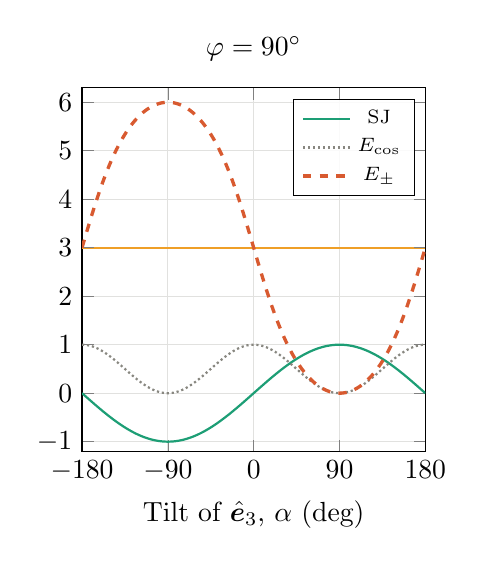
\begin{tikzpicture}
\begin{axis}[
  width=0.49\textwidth, height=6.2cm,
  title={$\varphi=90^\circ$},
  xmin=-180,xmax=180,ymin=-1.2,ymax=6.3,
  xtick={-180,-90,0,90,180},
  ytick={-1,0,1,2,3,4,5,6},
  xlabel={Tilt of $\uv{e}_3$, $\alpha$ (deg)},
  grid=major, grid style={slate!25},
  legend style={font=\scriptsize,at={(0.97,0.97)},anchor=north east,fill=white,fill opacity=0.85,text opacity=1},
  samples=241,domain=-180:180,
  extra y ticks={3}, extra y tick labels={}, extra y tick style={grid style={amber,thick}},
]
\addplot[teal,thick] {sin(90)*sin(x)};
\addlegendentry{$\SJ$}
\addplot[slate,thick,densely dotted] {cos(90)^2+2*cos(x)^2*cos(45)^2};
\addlegendentry{$\Eu$}
\addplot[coral,very thick,dashed] {3-sin(x)-2*sin(90)*sin(x)/sqrt(sin(45)^2+cos(45)^2*sin(x)^2)};
\addlegendentry{$\Es$}
\end{axis}
\end{tikzpicture}\hfill
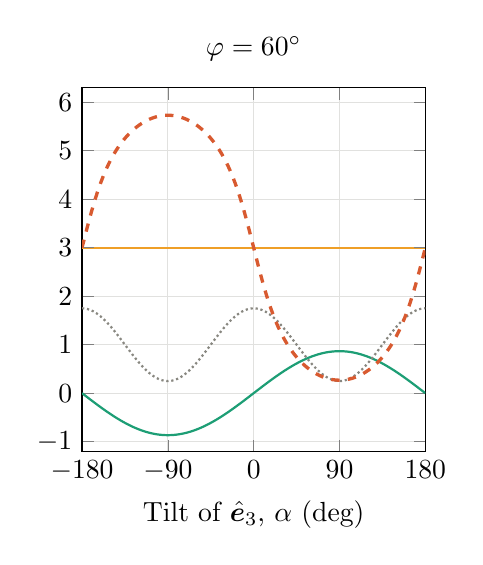
\begin{tikzpicture}
\begin{axis}[
  width=0.49\textwidth, height=6.2cm,
  title={$\varphi=60^\circ$},
  xmin=-180,xmax=180,ymin=-1.2,ymax=6.3,
  xtick={-180,-90,0,90,180},
  ytick={-1,0,1,2,3,4,5,6},
  xlabel={Tilt of $\uv{e}_3$, $\alpha$ (deg)},
  grid=major, grid style={slate!25},
  samples=241,domain=-180:180,
  extra y ticks={3}, extra y tick labels={}, extra y tick style={grid style={amber,thick}},
]
\addplot[teal,thick] {sin(60)*sin(x)};
\addplot[slate,thick,densely dotted] {cos(60)^2+2*cos(x)^2*cos(30)^2};
\addplot[coral,very thick,dashed] {3-sin(x)-2*sin(60)*sin(x)/sqrt(sin(30)^2+cos(30)^2*sin(x)^2)};
\end{axis}
\end{tikzpicture}
\caption{Scaled Jacobian, unsigned energy $\Eu$, and signed energy $\Es$ along the tilt sweep,
for a square base (left) and a skewed base (right). $\Es$ crosses the line $3$ exactly where $\SJ$
crosses $0$ and keeps rising through inversion; $\Eu$ turns back down and has a spurious second
minimum at the fully reflected corner $\alpha=-90^\circ$.}
\label{fig:curves}
\end{figure}

\begin{figure}[h]
\centering
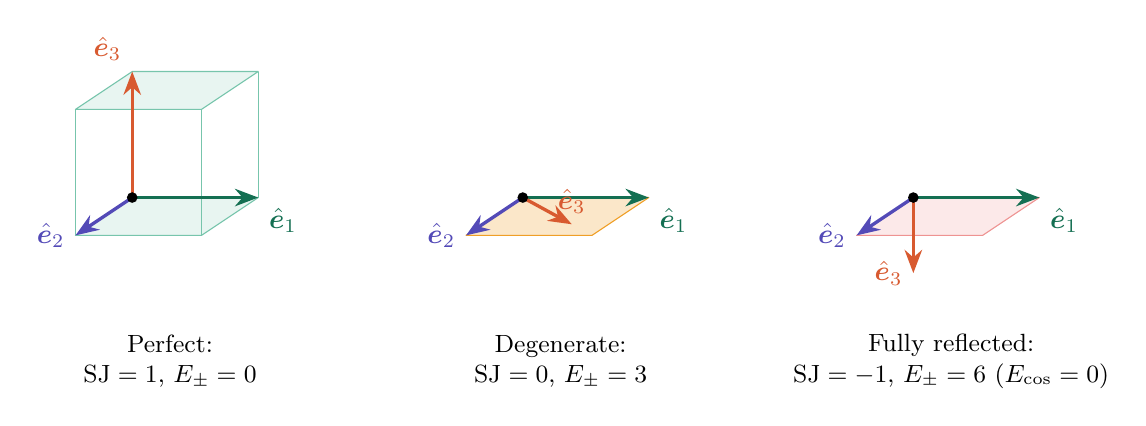
\begin{tikzpicture}[scale=1.6,line join=round,>=Stealth,x={(1cm,0cm)},y={(-0.45cm,-0.3cm)},z={(0cm,1cm)}]
  % perfect corner: e1=x, e2=y, e3=z
  \begin{scope}
    \coordinate (O) at (0,0,0);
    \coordinate (a) at (1,0,0);
    \coordinate (b) at (0,1,0);
    \coordinate (c) at (0,0,1);
    \coordinate (ab) at (1,1,0);
    \coordinate (ac) at (1,0,1);
    \coordinate (bc) at (0,1,1);
    \coordinate (abc) at (1,1,1);
    \filldraw[fill=teal!10,draw=teal!60] (O)--(a)--(ab)--(b)--cycle;
    \filldraw[fill=teal!10,draw=teal!60] (c)--(ac)--(abc)--(bc)--cycle;
    \draw[teal!60] (a)--(ac) (b)--(bc) (ab)--(abc);
    \draw[->,very thick,teal!70!black] (O)--(a) node[below right]{$\uv{e}_1$};
    \draw[->,very thick,purp] (O)--(b) node[left]{$\uv{e}_2$};
    \draw[->,very thick,coral] (O)--(c) node[above left]{$\uv{e}_3$};
    \fill (O) circle (1.2pt);
    \node[font=\small,align=center] at (0.3,0,-1.3) {Perfect:\\ $\SJ=1$, $\Es=0$};
  \end{scope}
  % degenerate corner: e3 in plane on the bisector
  \begin{scope}[xshift=3.1cm]
    \coordinate (O) at (0,0,0);
    \coordinate (a) at (1,0,0);
    \coordinate (b) at (0,1,0);
    \coordinate (c) at (0.707,0.707,0);
    \filldraw[fill=amber!25,draw=amber] (O)--(a)--(1,1,0)--(b)--cycle;
    \draw[->,very thick,teal!70!black] (O)--(a) node[below right]{$\uv{e}_1$};
    \draw[->,very thick,purp] (O)--(b) node[left]{$\uv{e}_2$};
    \draw[->,very thick,coral] (O)--(c) node[above]{$\uv{e}_3$};
    \fill (O) circle (1.2pt);
    \node[font=\small,align=center] at (0.3,0,-1.3) {Degenerate:\\ $\SJ=0$, $\Es=3$};
  \end{scope}
  % inverted corner: e3 points down
  \begin{scope}[xshift=6.2cm]
    \coordinate (O) at (0,0,0);
    \coordinate (a) at (1,0,0);
    \coordinate (b) at (0,1,0);
    \coordinate (c) at (0,0,-0.6);
    \filldraw[fill=redd!12,draw=redd!60] (O)--(a)--(1,1,0)--(b)--cycle;
    \draw[->,very thick,teal!70!black] (O)--(a) node[below right]{$\uv{e}_1$};
    \draw[->,very thick,purp] (O)--(b) node[left]{$\uv{e}_2$};
    \draw[->,very thick,coral] (O)--(c) node[left]{$\uv{e}_3$};
    \fill (O) circle (1.2pt);
    \node[font=\small,align=center] at (0.3,0,-1.3) {Fully reflected:\\ $\SJ=-1$, $\Es=6$ ($\Eu=0$)};
  \end{scope}
\end{tikzpicture}
\caption{Three corners of the test family with a square base. The unsigned energy $\Eu$ is zero
for both the left and right corners; the signed energy separates them.}
\label{fig:corners}
\end{figure}

\subsection{A simpler alternative and why it needs tuning}

One may instead keep $\Eu$ and add an orientation penalty,
\begin{equation}
  E_w=\Eu+w\,(1-\SJ),\qquad w>0.
\end{equation}
$E_w\ge0$ with equality only at the perfect corner (both terms must vanish, and $\SJ=1$ forces
orthonormal right-handedness by Proposition~\ref{prop:SJrange}). But monotonicity through
inversion depends on $w$. In the test configuration, using~\eqref{eq:SJconfig} and~\eqref{eq:Euconfig},
\begin{equation}
  E_w=\cos^2\varphi+2(1-s^2)h^2+w(1-s\sin\varphi),\qquad
  \frac{dE_w}{ds}=-4h^2s-w\sin\varphi.
\end{equation}
This is negative for all $s\in[-1,1]$ iff it is negative at the worst case $s=-1$:
\begin{equation}
  4h^2<w\sin\varphi
  \iff w>\frac{4\cos^2\frac{\varphi}{2}}{2\sin\frac{\varphi}{2}\cos\frac{\varphi}{2}}
  \iff \boxed{w>2\cot\frac{\varphi}{2}.}
\end{equation}
For a square base this needs $w>2$; for $\varphi=60^\circ$, $w>2\sqrt3\approx3.46$; for
$\varphi=20^\circ$, $w\gtrsim11.3$. The required weight grows without bound as the base collapses,
whereas $\Es$ is monotone for every $\varphi$ with no parameter to tune (Proposition~\ref{prop:mono}).

\subsection{Practical notes}

\begin{itemize}
  \item \textbf{Parallel edges.} $\uv{n}_{ij}$ is undefined when $\sin\theta_{ij}\to0$. Clamp
        $\|\uv{e}_i\times\uv{e}_j\|\ge\varepsilon$ in code. In an optimizer, it can help to keep a
        $\cos^2$ term alongside $\Es$, since $\cos^2\theta_{ij}$ remains smooth there.
  \item \textbf{Barriers versus finite penalties.} A barrier such as $-\log\SJ$ forbids inversion
        outright (it is infinite at $\SJ=0$). $\Es$ is finite everywhere, which is what one wants when
        an inverted mesh must be \emph{untangled} by descent: the gradient keeps pointing back toward
        validity on the inverted side.
  \item \textbf{Element energy.} An element energy can be formed as $\sum_{a=1}^{8}\Es^{(a)}$, or as
        $\max_a\Es^{(a)}$ to mirror the MSJ.
\end{itemize}

\subsection{Reference implementation}

\begin{lstlisting}[language=Python]
import numpy as np

CYCLIC = [(0, 1, 2), (1, 2, 0), (2, 0, 1)]

def corner_metrics(e1, e2, e3, eps=1e-12):
    """Return (SJ, E_cos, E_signed) for three edge vectors at a corner node.

    Edges must be ordered so that the reference frame is right-handed.
    """
    e = [np.asarray(v, float) / np.linalg.norm(v) for v in (e1, e2, e3)]
    sj = float(np.dot(np.cross(e[0], e[1]), e[2]))
    e_cos = sum(float(np.dot(e[i], e[j]))**2 for i, j in [(0, 1), (0, 2), (1, 2)])
    e_signed = 0.0
    for i, j, k in CYCLIC:
        n = np.cross(e[i], e[j])
        e_signed += 1.0 - float(np.dot(e[k], n)) / max(np.linalg.norm(n), eps)
    return sj, e_cos, e_signed
\end{lstlisting}

The closed forms~\eqref{eq:SJconfig}, \eqref{eq:Euconfig}, and~\eqref{eq:Esconfig} agree with this
vector implementation to machine precision ($\le 10^{-15}$) over a grid of
$\alpha\in[-180^\circ,180^\circ]$, $\varphi\in[20^\circ,160^\circ]$.

%=====================================================================
\section{Embedding interactive illustrations in an mdBook}
\label{sec:mdbook}
%=====================================================================

mdBook passes raw HTML through to the rendered page, so inline \verb|<svg>| and
\verb|<script>| work in any chapter. Three approaches, from simplest to most robust:

\begin{enumerate}
  \item \textbf{Inline HTML in the chapter.} Works, but the Markdown parser ends an HTML block at
        the first blank line, so the snippet---including the script---must contain no empty lines.
  \item \textbf{Markup in the chapter, code in a separate file (recommended).} Keep only a
        container in the chapter and register the script and stylesheet in \verb|book.toml|. The script
        locates every widget by class, so one widget can appear in several chapters or several times on a page.
  \item \textbf{An \texttt{<iframe>} to a standalone HTML page.} Fully isolated from mdBook's
        styles, but the height must be fixed by hand and it will not follow the reader's theme.
\end{enumerate}

\begin{lstlisting}[language=HTML,title={Chapter snippet (option 2)}]
<div class="dihedral-widget">
<svg viewBox="0 0 680 400" width="100%"><g class="scene"></g></svg>
<input type="range" min="10" max="180" value="110">
</div>
\end{lstlisting}

\begin{lstlisting}[title={book.toml}]
[output.html]
additional-js  = ["widgets/dihedral.js"]
additional-css = ["widgets/widgets.css"]
\end{lstlisting}

When porting widgets written for another host, replace host-specific CSS classes and variables
with mdBook's theme variables (e.g.\ \verb|var(--fg)| for text, \verb|var(--bg)| for background) so the
widget follows the Light, Rust, Coal, Navy, and Ayu themes. Hard-coded data colors (faces, edges,
arcs) can stay as they are.

%=====================================================================
\appendix
\section{Record of the conversation}
\label{app:conversation}
%=====================================================================

The user's requests are quoted verbatim; the assistant's responses are summarized.

\begin{enumerate}[label=\textbf{\arabic*.},leftmargin=*,itemsep=0.8em]
\item \textbf{User:} ``illustrate the dihedral angle between to triangular facets that share an edge''

\textbf{Assistant:} Produced an interactive 3D illustration: two triangular faces hinged on an
amber shared edge, dashed rays in each face perpendicular to the edge at a common point, a
coral arc marking $\theta$, a slider for $\theta\in[10^\circ,180^\circ]$, and drag-to-rotate. Explained
that viewing down the edge shows the true angle, and gave the normal-based formula
(Section~2).

\item \textbf{User:} ``wow, this is a very nice interactive illustration. Is there a way to include
such a nice interactive illustration in an mdbook?''

\textbf{Assistant:} Explained the three embedding options (inline HTML with no blank lines;
container markup plus \verb|additional-js|/\verb|additional-css| in \verb|book.toml|; an
\texttt{<iframe>}), recommended the second, and noted replacing host styles with mdBook theme
variables (Section~\ref{sec:mdbook}).

\item \textbf{User:} ``is there a second illustration you can create, of minimum Scaled Jacobian
for the the corner of a hexahedron of a finite element mesh with three incident edges at a single
node? I would love to be able to illustrate the MSJ going to zero and going negative, and how the
perfect MSJ of 1.0 looks.''

\textbf{Assistant:} Built an interactive hex corner: three edge vectors from a node, the unit
parallelepiped they span (colored green/amber/red for valid/degenerate/inverted), a live SJ
readout and a $[-1,1]$ gauge, sliders for the tilt of $\uv{e}_3$ and the angle between $\uv{e}_1$ and
$\uv{e}_2$, and presets (perfect, skewed, degenerate, inverted). Gave $\SJ=\sin\varphi\sin\alpha$ for
the configuration and described the three regimes (Sections~3--4).

\item \textbf{User:} ``is there a way to show `corner energy' as a B panel (A versus B panel) to the
hex, where the corner energy is zero for a perfect 90-90-90 degree corner, and then increases as
the angle between two axes separates from 90''

\textbf{Assistant:} Added panel~B plotting $\SJ$ and $\Eu=\sum\cos^2\theta_{ij}$ against the tilt,
next to the 3D corner in panel~A. Pointed out that $\Eu$ is blind to inversion: it falls back to $0$
for a fully reflected corner (Section~5).

\item \textbf{User:} ``is there a way to embed the sign of the corner in the corner energy such that
the corner energy continues to increase when the MSJ goes from zero to negative?''

\textbf{Assistant:} Explained that $\cos^2$ is even under reflection, so orientation must enter
through the oriented normal. Introduced $\Es=\sum_k(1-\uv{e}_k\cdot\uv{n}_{ij})=\sum(1-\SJ/\sin\theta_{ij})$,
with $\Es=0$ only at the perfect corner, $\Es=3$ exactly at $\SJ=0$, and $\Es>3$ when inverted.
Updated panel~B with all three curves. Noted the parallel-edge guard and the alternative
$\Eu+w(1-\SJ)$, which needs $w\ge2\cot(\varphi/2)$ (Section~6).

\item \textbf{User:} ``For the x-axis `Tilt of e\_3', it current runs from -60 deg to 90 deg. Can we
make that axis run from -180 degrees to 180 degrees?''

\textbf{Assistant:} Extended the slider and axis to $[-180^\circ,180^\circ]$ and the energy axis to
$[-1,6]$, added a ``fully reflected'' preset at $-90^\circ$, and reported separate $\theta_{13},\theta_{23}$
and $\psi_3$. Over the full sweep, $\SJ$ is a sine wave; $\Eu$ has two equal minima at
$\pm90^\circ$; $\Es$ has a single minimum at $+90^\circ$, a single maximum at $-90^\circ$, and crosses
$3$ exactly where $\SJ=0$ (Figure~\ref{fig:curves}).

\item \textbf{User:} ``can you write down this entire conversation, along with a formulation, into a
LaTeX .tex document I can download, please include all the derivations of the formulae.''

\textbf{Assistant:} Produced this document.
\end{enumerate}

\end{document}
